\documentclass[10pt,sigconf]{acmart}
\settopmatter{printacmref=false} % Removes citation information below abstract
\renewcommand\footnotetextcopyrightpermission[1]{} % removes footnote with conference information in first column
\pagestyle{plain}
\usepackage[english]{babel}
\usepackage{blindtext}



\begin{document}
\title{A \LaTeX\ Template for HTDN 2020}

\subtitle{Fancy subtitle}
 \author{Amirhossein Saemi}
% \authornote{Note}
% \orcid{1234-5678-9012}
% \affiliation{%
%   \institution{Affiliation}
%   \streetaddress{Address}
%   \city{City} 
%   \state{State} 
%   \postcode{Zipcode}
% }
 \email{amsa00004@uni-saarland.de}


\begin{abstract}
In a time where television and radio no longer dominate as the sole forms of mass communication, the Internet emerges as a significant potential adversary to the spread of propaganda. Consequently, world governments often strive to develop technologies that allow them to exert control over the internet and maintain their monopoly as information empires. 

While censorship may not be a new concept, it remains an effective tool in combating the spread of undesirable information. This paper examines the development of Internet censorship and how users have countered it by employing different circumvention tools. A specific focus is placed on the examination of the Great Firewall of China and how it detects fully encrypted traffic in real-time. Despite the GFW's blackbox nature, we explore how supporters of a free Internet have developed novel escape strategies based on GFW's observed behavior when probing with specially crafted payloads.

Next, we explore how and why world governments make use of a variety of techniques in parallel to exert greater control over the Internet. Ultimately, we conclude our review by advocating for the automation of censorship circumvention through collaborative machine analysis and artificial intelligence.
\end{abstract}

\maketitle

\section{Introduction}
Censorship techniques are evolving alongside the expansion of the internet, with governments employing complex and expensive methods such as Deep Packet Inspection. DPIs utilize stateful censorship which involves maintaining connection state information. Although expensive, this kind of censorship offers advanced analysis capabilities to achieve better control over internet users which wasn't previously possible using basic techniques such as DNS poisoning or IP blocking. Such DPIs usually distinguish circumvention traffic by identifying unique fingerprints of different internet protocols.

In response to the evolving censorship techniques, circumvention tools have equally evolved and are prepared to combat censorship. One effective strategy they employ is to camouflage themselves within the vast sea of legitimate HTTPS traffic. Such techniques often rely on mimicking an allowed protocol (e.g. Skype) as a means to become unobservable and remain unnoticed by the censor.

\section{Related Work}
While most of the current circumvention protocols rely on mimicking to remain unnoticed by the censor, some authors believe that the entire approach of “unobservability by imitation” is fundamentally flawed and argue that mimicking a sophisticated distributed system like Skype, with multiple, inter-dependent sub-protocols and correlations, is an impossible challenge. Hence, a parrot circumvention protocol may not fully align its protocol with the actual protocol, leading to being easily detectable by censors. They believe that one promising alternative is to not mimic, but run the actual protocol instead.\cite{houmansadr2013parrot}

Other solutions proposed by researchers suggest moving the proxying logic from the edge (the proxy server) to the core of the network outside the censored regime. Such solutions are usually deployed by friend ISPs and help to obfuscate the origin/destination of packets, usually referred to as Decoy Routing. An example of such implementation is the Cirripede Circumvention Infrastructure.[cite] While decoy routing is a novel idea, its effectiveness against DPIs with content analysis capabilities is under question.\cite{karlin2011decoy}\cite{houmansadr2011cirripede}

Finally, a promising work done by Wang et al. is to interfere with the state management of the censor by exploiting the fact that any Network Intrusion Detection System (NIDS) is inherently incapable of always reconstructing a TCP stream the same way as its endpoints, and have shown that a sender can send carefully crafted packets to desynchronize the TCP Control Block (TCB) maintained by the NIDS tricking it into forgetting about monitoring a specific live connection. Since the GFW is inherently a NIDS, the client could easily evade the real-time censor by employing this method.\cite{wang2017state}

\section{Background}
\begin{figure}[tp]
	\centering
	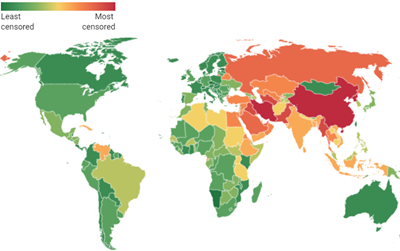
\includegraphics{figures/WorldCensorship}
	\caption{
		Which countries are the most censored in the world?
		\cite{comparitech2023}
	}
\end{figure}

\subsection{Evolution of Censorship Techniques}
In parallel with the continuous expansion of internet users, diverse web services and social media apps that have become integral to modern life, censorship techniques are also actively evolving by world governments. 

As a response, the anti-censorship community is committed to developing and distributing circumvention tools for accessing the unrestricted Internet. Consequently, governments have shifted from simple and cost-effective approaches to more complex, expensive, and harder-to-circumvent censorship techniques.

These methods vary from simple DNS poisoning to advanced technologies like Deep Packet Inspection (DPI), allowing them to make decisions on a per-connection basis. In extreme cases, certain countries are even willing to pay astronomical prices, resorting to complete internet shutdowns.

Some countries have taken further steps by developing tools to weaponize innocent users, turning them into botnets used for attacking and disrupting popular VPN service providers. China's Great Canyon is a specific example, where malicious JavaScript payloads are sent to users to perform DDoS attacks on targeted websites.\cite{marczak2015great}

\subsection{From Centralized to Distributed Censorship Control}
Given the decentralized structure of the Internet, it is impractical to route the entire traffic of a country through a single device or a cluster of censoring devices. Instead, each Internet Service Provider (ISP) is responsible for implementing censorship individually, ideally at the network edge. The management of these middleboxes can be established either centrally, directly by authorities, or individually by each ISP, depending on their respective policies.

In some countries, like Russia, a centralized control model is implemented, where the authority maintains control over a network of numerous Internet Service Providers (ISPs). This centralized approach grants substantial power to the authorities, allowing them to unilaterally impose desired restrictions. In contrast, countries such as Iran follow a distributed model, resulting in potential inconsistencies in censorship behavior among different ISPs, leading to varied experiences for users.\cite{xue2021throttling}

In India, the authorities shared that while the censorship policies are confidential, the onus of implementing them lies with the individual ASes who could employ any mechanism they choose.\cite{yadav2018light}

While a centralized approach may offer a faster response and the ability to swiftly implement blocks, distributed control could prove more resilient in combating constantly updated circumvention tools. This is because circumvention tools must take into account the diverse policies and technologies employed by different ISPs in a distributed model.

\subsection{Stateful Censorship}
To examine the application-layer content with DPI, a censorship system like the GFW needs to keep some state to track each TCP connection. In particular, it maintains a TCP Control Block (TCB) for each live connection to track its state information (e.g., TCP state, sequence number, acknowledgment number, etc.). The goal is to replicate the same connection information at both endpoints. \cite{wang2017state}

While not all censorship techniques necessitate maintaining state, stateful censorship, despite its costliness, offers significant flexibility and advanced analysis capabilities. However, using specially crafted packets makes it possible to desynchronize the state on the DPI and evade the censor without disrupting the client or the server.

\subsection{Circumvention Technologies}
In the early phases of internet censorship, blocking mostly took place at the routing layer, utilizing IP blacklists and whitelists to limit access to particular IP addresses/ranges. However, users quickly discovered they could leverage the network as a simple proxy service, leveraging multiple access points to evade basic IP/Port blocking. These techniques involved encapsulating packets within another packet and requesting a proxy server to transmit the inner packet to the intended destination and vice versa.

The advent of Deep Packet Inspection (DPI) systems with content-based filtering capabilities rendered the previous approach ineffective. However, users soon discovered that encrypting packets became a valuable solution as the DPI could no longer comprehend the content within.\cite{leberknight2010taxonomy}

Various protocols such as Tor found success at that time. However, Tor’s biggest weakness in this respect is its global public list of relays where a censor can simply download and add each IP address to a blacklist - and censors began to do exactly that. In response to blocking its relays, Tor began to carefully distribute bridges through rate-limited out-of-band channels (such as email or HTTP). This makes it possible for everyone to learn a few bridge addresses while making it hard for anyone to learn them all.

Even using secret bridge relays, Tor remains vulnerable to detection by deep packet inspection (DPI). Tor uses TLS in a fairly distinctive way that causes it to stand out from other TLS-based protocols. After early efforts to make their use of TLS less conspicuous, the developers of Tor settled on a more sustainable strategy: wrapping the entire Tor TLS stream in another layer—a “pluggable transport” and shortly after, transport protocols Obfs2, Obfs3, and Obfs4 were introduced.\cite{ensafi2015firewall}

\section{Mechanics of Real-time Censorship in GFW}
Content of this section is mostly a summary of the work done by Wu et al. (2023) with some minor changes  and possible re-orderings.\cite{wu2023great}

\subsection{Protocol Fingerprinting}
Every internet protocol has its distinct characteristics that differentiates it from other protocols. This knowledge enables censors to recognize circumvention traffic by detecting these unique fingerprints. Censors develop regular expressions specifically designed to identify indicators of permissible traffic, allowing them to quickly exempt such traffic from censorship and classify it as allowed.

For instance, in 2012, China and Ethiopia deployed deep packet inspection to detect Tor traffic by its uncommon ciphersuits. Censorship middlebox vendors have previously identified and blocked meek traffic based on their TLS fingerprint and SNI values.\cite{wu2023great}

Before the implementation of the new censorship system by the GFW, fully encrypted traffic was generally treated as regular traffic, likely because the GFW was cautious about the potential collateral damage caused by mistakenly blocking legitimate traffic. This conservative approach might have reflected the GFW's uncertainty in having collected fingerprints for all the allowed protocols.

With the implementation of the new censorship system, the effectiveness of fully encrypted tunnels came into question. Even though an encrypted tunnel leaks no information about the payload or its final destination, it still requires effort to perfectly align its fingerprints with popular protocols that form the majority of traffic to avoid blocking.

An important characteristic of fully encrypted traffic that differentiates it from other traffic is its high entropy homogeneously throughout the entire connection, even in the first data packet. Because fully encrypted traffic is supposed to be purely random, it will have close to half of the bits set to 1. This is in contrast to other protocols with fewer than 1 bits per byte due to plaintext or zero-padded protocol headers.\cite{wu2023great}

\subsection{Flow Reassembly}
It is observed that a complete TCP handshake is necessary to trigger the real-time censor. Also, the GFW only examines the first data packet for now. Moreover, it is shown that the GFW waits more than 5 minutes for the first data packet. However, it is worth mentioning that only client-to-server packets can trigger the blocking; The server here is defined as the host that sends a SYN+ACK during the TCP handshake.\cite{wu2023great}

A potential approach to bypass real-time censorship would involve sending the first packet in a way that convinces the censor it is part of an allowed traffic flow while sending circumvention traffic in the subsequent packets. The server would be expected to disregard the first packet accordingly. However, the censor could easily change its behavior to check packets other than the first one with the help of its stateful nature.

The evasion strategy must ensure that there are no conspicuous fingerprints that would indicate the presence of forbidden traffic to the censor.

\subsection{How the GFW Disrupts a Connection}
Once the GFW detects fully encrypted traffic, it aims to drop client packets accordingly, indicating that only client-to-server packets are affected. At this stage, the client does receive server responses.

Interestingly, this type of censorship specifically impacts TCP connections, as sending the same triggering packet over UDP does not alter its behavior. One possible explanation is that implementing UDP censorship might require additional resources and introduce added complexity.

Furthermore, it's important to note that not all ports are immune to being blocked. Using a sink server that listens on all ports reveals that the censor can be triggered on any destination port.

Moreover, an internet scanning experiment demonstrates that the impact of censorship is not uniform across all subnets/ASes. Even within each AS, different prefixes are treated differently. Notably, the affected or partially affected ASes primarily comprise popular VPS providers that could potentially be used to host proxy servers. Conversely, unaffected ASes typically do not offer VPS hosting services to individual customers.\cite{wu2023great}

\subsection{Residual Censorship}
After a connection triggers the censorship, the GFW blocks all subsequent connections having the same 3-tuple (client IP, server IP, server port) for 180 seconds.\cite{wu2023great}

During this period of 180 seconds, no additional handshakes to the same 3-tuple will be possible. This can be particularly valuable for confirming whether a specific payload has triggered censorship. Nevertheless, assuming the server is a sink server, other ports on the same server remain accessible for testing with different crafted payloads. 

\subsection{Probabilistic Blocking}
The GFW employs a probabilistic blocking strategy, where censorship is only triggered approximately a quarter of the time.

This is taken into account when testing if a particular payload triggers the censor by sending the same payload in up to 25 connections before concluding. If after sending the payload at least once, a sequence of 5 subsequent connection attempts timeout (due to residual censorship), the payload (and server) are then labeled as affected by censorship, and the 3-tuple will not be used for 180 seconds. 

Conversely, making 25 consecutive successful connections with the same payload indicates that the censor is not triggered. This method is effective in avoiding false negatives when probabilistic blocking is employed.\cite{wu2023great}

\section{Evading Real-time Censorship}
Content of this section is a summary of the work done by Wu et al. (2023) with some minor changes and possible re-orderings.\cite{wu2023great}

\subsection{Detecting Exemption Rules}
To develop effective evading strategies, it is crucial to understand how the Great Firewall defines and identifies allowed traffic. Armed with this knowledge, it is possible to employ a steganographic approach by modifying evasion packets to resemble permitted traffic. This technique involves hiding circumvention traffic within the outward appearance of authorized traffic, making it more challenging for the GFW to detect and block. 

To accomplish this, Wu et al. (2023) employed the following experimental setup to extract the rules utilized by the Great Firewall for exempting authorized traffic:

\textbf{Multiple Vantage Points.} The experiment involved the use of ten VPSes in TencentCloud Beijing and one VPS in AlibabaCloud Beijing. Additionally, four VPSes in DigitalOcean San Francisco were utilized, three of them being affected by new censorship. These VPSes were transformed into sink servers, accepting TCP connections but not sending any data back.

\textbf{Crafted Payloads.} The study employed crafted payloads as part of the research methodology. Alongside using genuine circumvention tools, measurement tools were created to trigger blocking. These tools would initiate a TCP handshake, transmit a random payload of a specified length, and then terminate the connection. The impact of each payload was then further examined by checking for any residual censorship indicators.

\textbf{Accounting for Probabilistic Blocking with Repeated Tests.} Due to the probabilistic blocking strategy employed by the GFW, censorship is triggered only about 25\% of the time. To accommodate this probabilistic behavior, the identical payload is sent in up to 25 connections before drawing any conclusion.


\subsection{Discovered Rules}
Wu et al. (2023) discovered that through the repeated sending of various payloads, they were able to deduce certain detection rules employed by the Great Firewall (GFW) to exclude permitted traffic. However, the researchers remain uncertain about the specific sequence in which these rules are applied or whether they are exhaustive. It was observed that rather than directly defining fully encrypted traffic, the censor utilized at least five heuristics to effectively exempt traffic that is unlikely to be fully encrypted. These exemption rules are derived from common protocol fingerprints. In this section, we will closely examine each of these rules to gain a better understanding of how they operate.

\subsubsection{\textbf{Entropy Exemption (Ex1)}}
During the observation, it was noticed that the likelihood of a connection being blocked is influenced by the fraction of bits set in the transmitted data. To investigate this further, a series of experiments were conducted where multiple connections were sent to the server and the blocked ones were identified. Each connection involved the transmission of one of 256 different byte patterns, with a single byte repeated 100 times (e.g., \textbackslash x00\textbackslash x00\textbackslash x00..., \textbackslash x01\textbackslash x01\textbackslash x01..., ..., \textbackslash xff\textbackslash xff\textbackslash xff...). These patterns were sent in 25 connections, and it was observed whether any of them triggered subsequent blocking.

Out of the 256 patterns, it was found that 40 patterns resulted in blocking, while the remaining 216 patterns did not lead to blocking. The blocked patterns had a common characteristic: the bytes consisted of exactly 4 out of 8 bits set to 1 (e.g., \textbackslash x1b in binary is 00011011). This observation led to the hypothesis that the number of set bits per byte, or the density of 1s, could play a role in triggering blocking. The reasoning was that uniformly random data would have a roughly equal number of 1s and 0s in binary representation, indicating a certain level of entropy within the packet's bits.

Of course, random or encrypted data will not always have exactly half of the bits set to 1. It was tested how close to half the GFW needed in order to block, and it was found that all strings with $\leq$ 3.4 or $\geq$ 4.6 bits/byte set were not blocked, while strings with between 3.4 and 4.6 bits/byte set were blocked.

\subsubsection{\textbf{First six bytes are printable (Ex2)}}
It is observed that the GFW exempts blocking if the initial six bytes of a connection fall within the printable byte range 0x20–0x7e. If there exist characters outside this range in the first six bytes, a connection may be subject to blocking, unless it possesses other exempting properties (e.g., fewer than 3.4 bits per byte set). To test this, messages were generated with the first n bytes originating from various character sets, such as ASCII printable characters, while the remaining part of the message consisted of random unprintable characters. It was discovered that for n $\textless$ 6, censorship was observed, whereas, for n $\geq$ 6, where the first n bytes are ASCII printable characters, no blocking occurred.

\subsubsection{\textbf{Half of the first packet are printable (Ex3)}}
If over half of the bytes in the initial packet fall within the printable ASCII range of 0x20–0x7e, the GFW exempts the connection. To ensure that the testing probes do not trigger other rules, precautions are taken. The probes are specifically designed to avoid triggering additional GFW exemptions, such as bit counts (Ex1), printable prefixes (Ex2), or runs of printable characters (Ex4). 

There's no wonder that the GFW allows plaintext, as its content can be easily inspected and understood by anyone who intercepts it.

\subsubsection{\textbf{More than 20 contiguous bytes are printable (Ex4)}}
A contiguous run of printable characters can also exempt blocking, even if the overall fraction of printable characters is less than half. It was observed that when n is less than or equal to 20, the connection was blocked. However, for n greater than 20, the connection was not blocked, indicating that the presence of a run of printable characters exempts blocking.

The study examined whether Chinese characters in the initial packet received the same blocking exemptions as printable ASCII characters. Both UTF-8 and GBK encoded strings containing Chinese characters were tested, but no exemptions were observed. These results suggest that Chinese characters do not enjoy any special exemptions. One possibility is that Chinese characters are infrequently encountered in these encodings. Additionally, parsing these encodings introduces complexities as it becomes challenging to determine the precise starting and ending points of an encoded string.

\subsubsection{\textbf{Common Protocols Exemption (Ex5)}}
To avoid blocking popular protocols by mistake, the observation is made that the GFW explicitly exempts two widely used protocols. The GFW appears to determine protocols based on the initial 3-6 bytes of the client's packet. If these bytes match those of a known protocol, the connection is exempted from blocking, even if the remaining packets do not adhere to the protocol. It has been found that the TLS and HTTP protocols are specifically exempted.

Testing was conducted on other commonly used protocols. SSH, SMTP, and FTP would also be exempted since they all begin with at least 6 bytes of printable ASCII (referred to as rule Ex2). DNS-over-TCP is exempted due to a significant number of zeros present, which qualifies for exemption under rule Ex1. However, if a substantial amount of random data is appended to a DNS-over-TCP message, it would be subject to blocking.

This observation raises the question of why the censor applies explicit rules to exempt TLS and HTTP, while other protocols do not receive the same treatment. The censor may employ these simple but efficient rules to quickly exempt the bulk of traffic (TLS and HTTP) from the more in-depth analysis of calculating the popcount, fraction of ASCII, etc.

\subsection{Evaluating Discovered Rules}
To determine the impact this blocking may have on regular traffic, the inferred detection rules are simulated on traffic on the university network without actually blocking any traffic. Different from the GFW, the detection rules are simulated against all TCP connections observed without limiting the detection to 26\% of connections to specific IP ranges of popular data centers. It is expected to see little to no circumvention traffic in this network, and any traffic that would be blocked under detection rules likely represents false positive blocking. The findings indicate that the inferred detection algorithm would block roughly 0.6\% of all connections on the network, suggesting good coverage of what the GFW uses by the inferred rules.

\subsection{Circumvention Strategies}
In this section, we introduce two widely adopted countermeasures that have been helping users in China bypass censorship since January 2022 and October 2022.

\textbf{Customizable Payload Prefixes.} Exemption rules Ex2 and Ex5 solely examine the initial bytes in a connection, enabling the GFW to efficiently exempt non-fully encrypted traffic. However, this approach presents a potential vulnerability. Nonetheless, a potential evasion tactic involves adding a customizable prefix to the payload of the initial packet in a circumvention connection. An effective illustration of this approach is allocating the first six bytes of the IV header in Shadowsocks protocols as printable ASCII. Implementing these countermeasures necessitates minimal modifications to the client and no adjustments to the server. Nevertheless, it's important to note that this is a temporary solution and the censor could potentially block it with relative ease.

\textbf{Altering Popcount.} The GFW exempts a connection if its first data packet has an average popcount-per-byte ${\leq}$ 3.4 or ${\geq}$ 4.6 (Ex1). Based on this observation, one can increase (or decrease) the popcount ratio by inserting additional ones (or zeroes) into the packet to bypass censorship.

By operating only on the ciphertexts, it does not risk violating confidentiality. When sending a packet, the average popcount-per-byte is computed first, and then the appropriate padding is added along with 4 bytes denoting the number of bits added. This process results in a bit-string B that has a popcount-per-byte that would not subject it to censorship.

Of course, simply appending ones or zeroes would be easy to fingerprint. To address this, bit-level random shuffling is employed. In particular, existing shared secrets, such as a password, are used as a seed to deterministically construct a permutation vector used for shuffling/unshuffling the bit-string. Since it is an obvious fingerprint if all connections share the same popcount-per-byte value, the popcount ratio value is set to a parameterizable range.

\section{Combining Multiple Censoring Techniques}
The internet undeniably presents a vast attack surface, and governments often exploit it to exert greater control. To achieve their objectives, governments usually employ multiple censoring techniques concurrently. This approach serves several purposes. Firstly, it reduces the strain on each censoring strategy, ensuring a more efficient censorship process. Additionally, employing a variety of techniques allows for broader coverage of circumvention technologies, tightening the avenues of escape from censorship. Economically, governments can reduce costs by utilizing cheaper technologies for handling bulk traffic while reserving more advanced methods for targeting high-tech circumvention tools. Moreover, this multi-faceted approach helps mitigate the risks associated with relying solely on a single censoring technique. Governments perceive this as an ongoing arms race, constantly preparing themselves for the emergence of new and innovative circumvention tools.

\subsection{The Role of Active Prober}
One such tool is China's active prober, which runs in parallel with the GFW. The active prober is designed to detect privacy tools and has proven particularly effective in targeting circumvention means such as Tor. It employs a combination of passive monitoring and active probing techniques to identify suspicious traffic and subsequently investigate corresponding servers. For this purpose, the prober hijacks real user IP addresses when sending probes, ensuring a stealthy approach. During testing, it sends arbitrary payloads to the target server, checking for responses that indicate the use of forbidden protocols such as Tor. The prober mimics user behavior, making it difficult to distinguish from genuine users during the probing phase. Once suspicions are confirmed, the server IP is appended to a blacklist.\cite{ensafi2015firewall}

To defend against the prober's activities, it is helpful to identify and avoid the factors that trigger its actions during passive monitoring. Furthermore, analyzing server logs can provide valuable insights into understanding what has attracted the prober as well. The prober actively probes for various protocols, including TLS, Tor Obfs2, Tor Obfs3, SoftEther, etc. Requiring clients to prove knowledge of a shared secret before responding could be another defense against the active prober.\cite{ensafi2015firewall}

Wu et al. (2023) found that the active probing system also relies on the traffic exemption rules introduced in section 5 but has additional packet length-based rules applied. They also showed evidence that the traffic analysis algorithm used by the active probing system may have evolved since 2019.\cite{wu2023great}

\begin{figure}[tp]
	\centering
	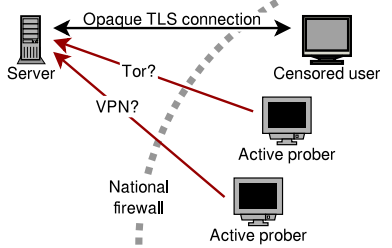
\includegraphics{figures/ActiveProber}
	\caption{
		The firewall cannot determine, by mere inspection, whether the encrypted connection carries a prohibited circumvention protocol. Therefore it issues its own probes and observes how the server responds.\cite{ensafi2015firewall}
		}
\end{figure}

\section{Other Examples}
While China is particularly famous for the GFW, it is not the only country turning up the heat. There are many more countries following China's footsteps using various censoring methods. In this section, we examine a non-exhaustive list of censoring countries studied by this article.

\textbf{Russia.} Apart from blocking websites, Russia is known to be the first government to apply bandwidth throttling on a national level for censorship. The slowdown was intended to pressure Twitter to comply with content removal requests from the Russian government. Throttling in Russia is achieved by exploiting the exposed domain name within the ClientHello message of the TLS protocol. Finally, under pressure, Twitter fulfilled the majority of content takedown requests to comply with the Russian government’s order without providing any transparency to its users.\cite{xue2021throttling}\cite{chai2019importance}

\textbf{Iran.} Iran has a long history of blocking, throttling, and shutting down the Internet. Apart from common censoring techniques such as DNS poisoning, IP blocking, and keyword filtering, Iran also utilizes DPIs to have finer control over the use of privacy tools.\cite{aryan2013iran}

\textbf{India.} Although censorship practices vary among different ISPs in India, there has been a gradual and somewhat covert development of an infrastructure for widespread Internet censorship. This infrastructure involves both privately and federally operated ISPs. Researchers who have sought further information from authorities have received nothing but vague and ambiguous responses.\cite{yadav2018light}

\textbf{Italy.} It is alarming to note that censorship has extended its reach to Europe. Reports suggest that Italy has resorted to utilizing DNS poisoning, leading to the failed resolution of several domains.\cite{aceto2017italy}

\section{Conclusion}
The ongoing conflict between censors and circumvention tools is indeed an arms race. With each side updating their strategies, the other side swiftly responds with countermeasures. While the circumvention community diligently safeguards the rights of citizens, there is a certain delay in restoring internet access whenever the censor's tactics are updated.

Undoubtedly, the censor operates as a black box, making it challenging to understand its inner workings. Nevertheless, conducting fuzzing tests on the DPI censor often uncovers valuable insights about its behavior. 
To begin with, it is essential for circumvention tools to store their knowledge of the network's state in a public repository where researchers can analyze the results. This collaborative approach allows for a collective pool of knowledge about what is allowed by the censor.

Subsequently, the gathered results should be analyzed to conclude the types of packets that are permitted to pass through the censor at any given time. While network analysts typically perform this step, it is worth noting that humans are significantly slower than machines when it comes to analyzing the results. Therefore, leveraging machine analysis can greatly expedite the process and enhance the efficiency of drawing insights from the shared data. The utilization of AI technology holds immense potential in extracting patterns utilized for constructing new escape routes from the censor. 

Finally, the client application should be designed to select the most suitable escape strategy based on the specific situation, thereby empowering users with the most effective circumvention strategies.

\bibliographystyle{ACM-Reference-Format}
\bibliography{reference}

\end{document}
